\section{Escenarios}

\subsection{Crear Equipo}

En el siguiente escenario unParticipante crea un equipo eligiendo con el nombre Pipe\&Filter, el tecnico Popovich, el base LeBron James,escolta Kevin Durant, alero ShaquilleONeal, ala pivot Michael Jordan y como pivot Kobe Briant. 
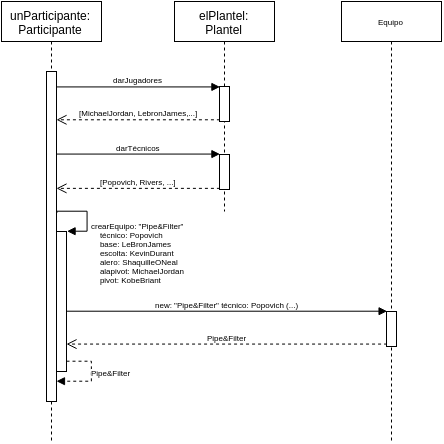
\includegraphics[width=\textwidth]{imgs/crearEquipoSecuencia.png}

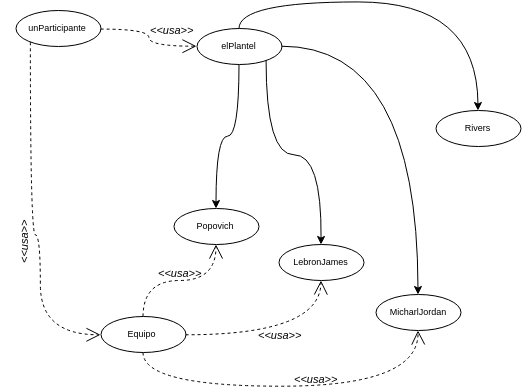
\includegraphics[width=\textwidth]{imgs/crearEquipoObjetos.png}



\subsection{Aceptar Desafío}
En este escenario otroParticipante elige de un pool de Desafíos el desafío donde está el equipo Pipe\&Filter apostando 5 fichas y lo acepta con su equipo llamado Batch. Luego el partido se simula y gana el equipo Pipe\&Filter 97 a 92 generando una ganancia de 15 fichas para unParticipante y una perdida de 5 fichas para otroParticipante. 

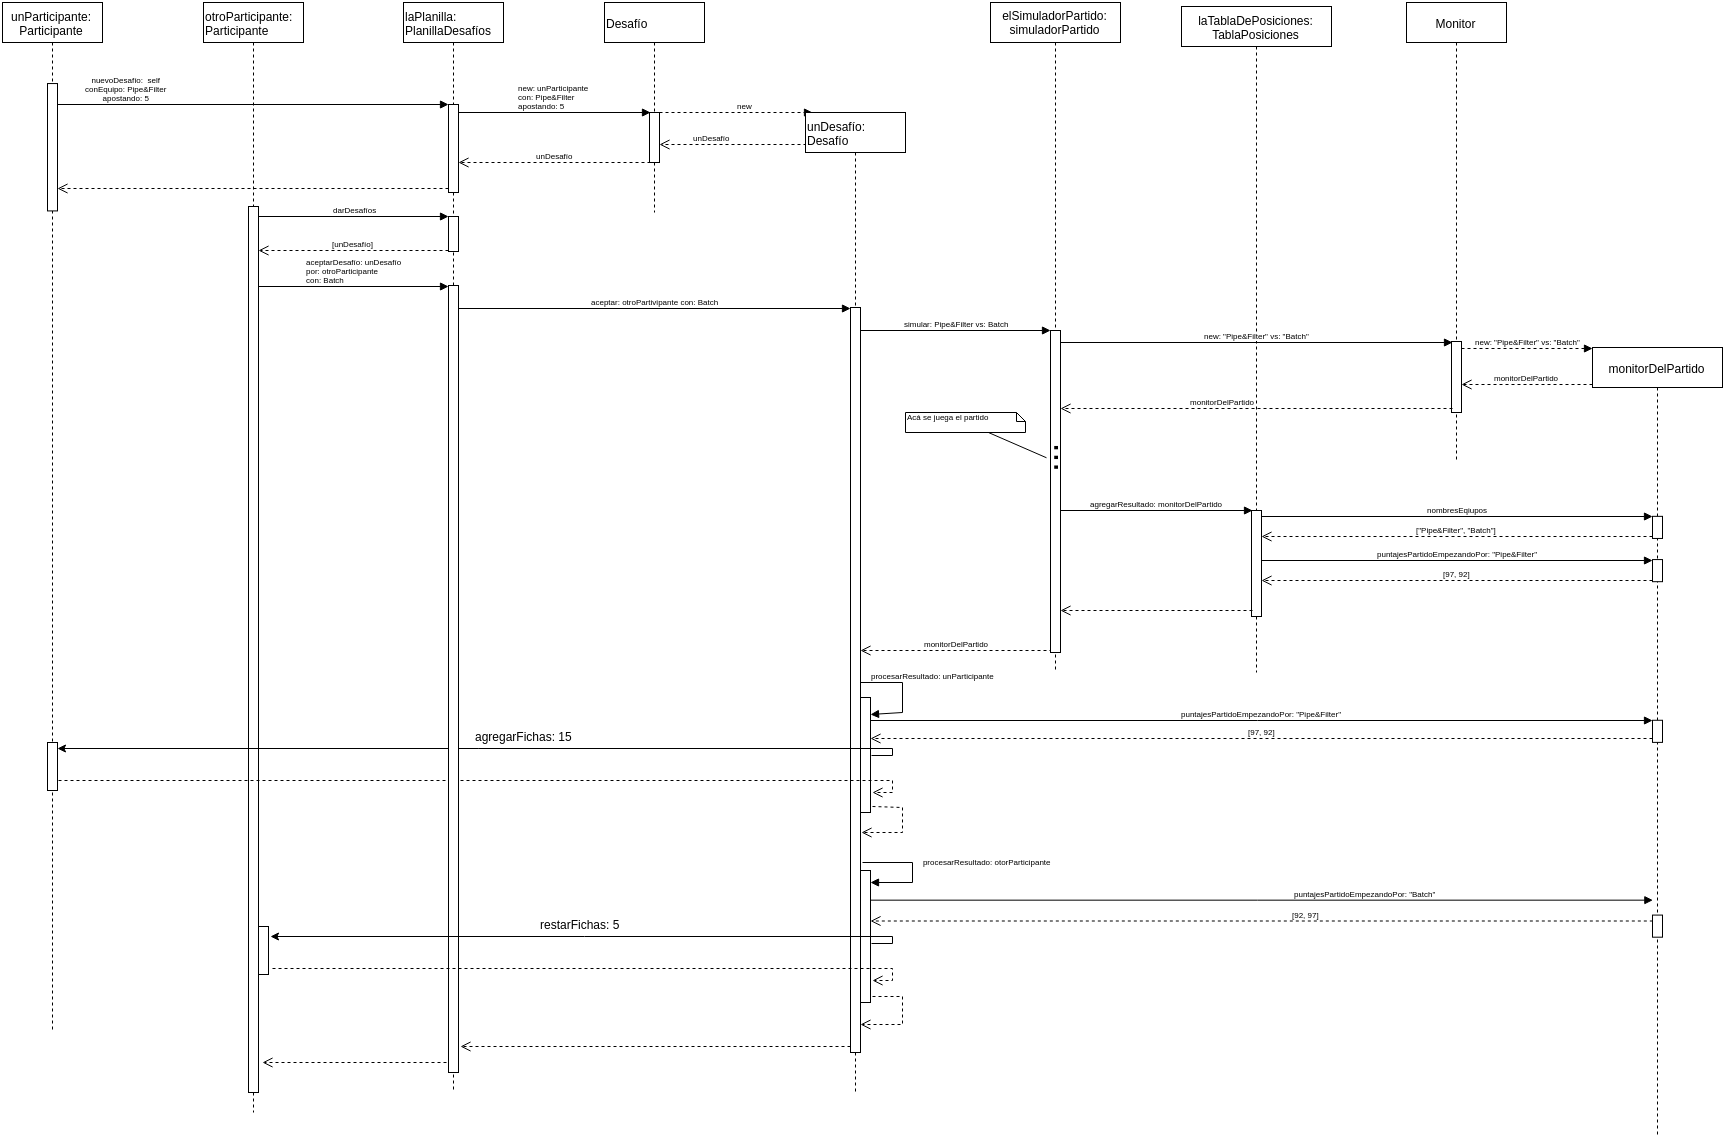
\includegraphics[width=\textwidth, angle =90 ]{imgs/aceptarDesafioSecuencia.png}

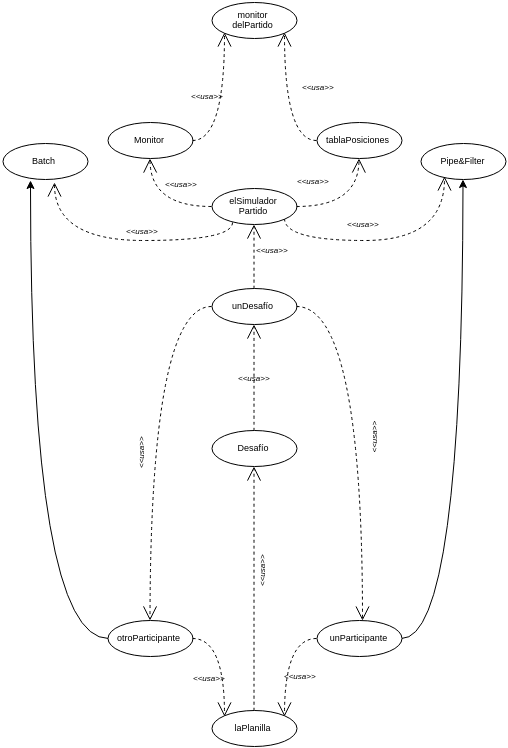
\includegraphics[width=\textwidth]{imgs/aceptarDesafioObjetos.png}

\subsection{Pase Exitoso}

El siguiente diagrama muestra una secuencia de mensajes de un pase que es exitoso. Esta secuencia estará en las simulaciones del simuladorDeTurno.

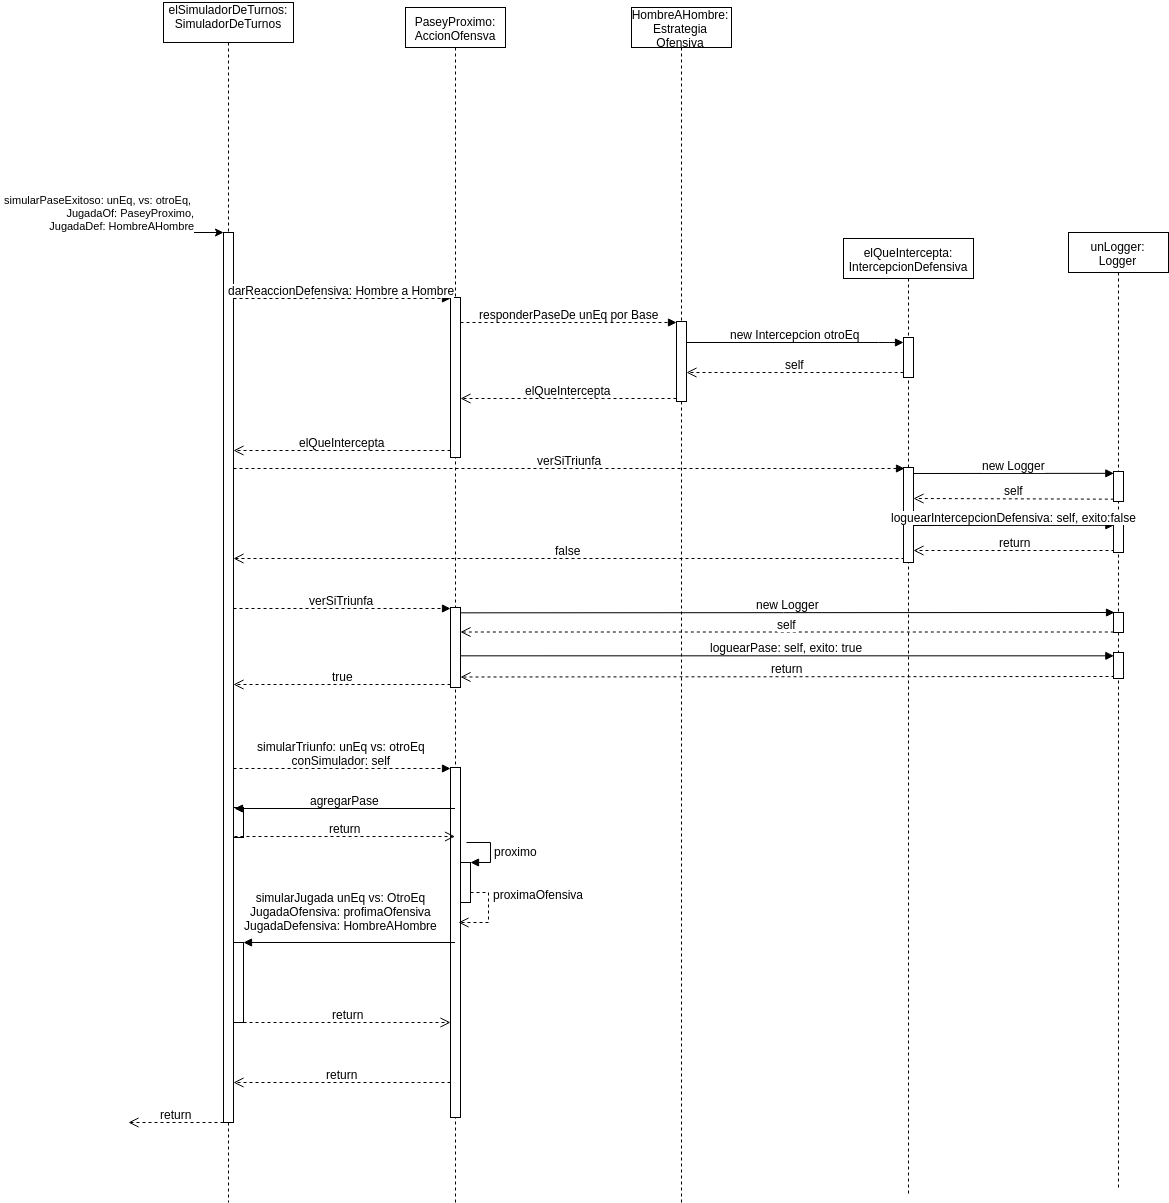
\includegraphics[width=\textwidth]{imgs/PaseExitoso.png}

\subsection{Pase Fallido}

Análogamente para el Pase Fallido

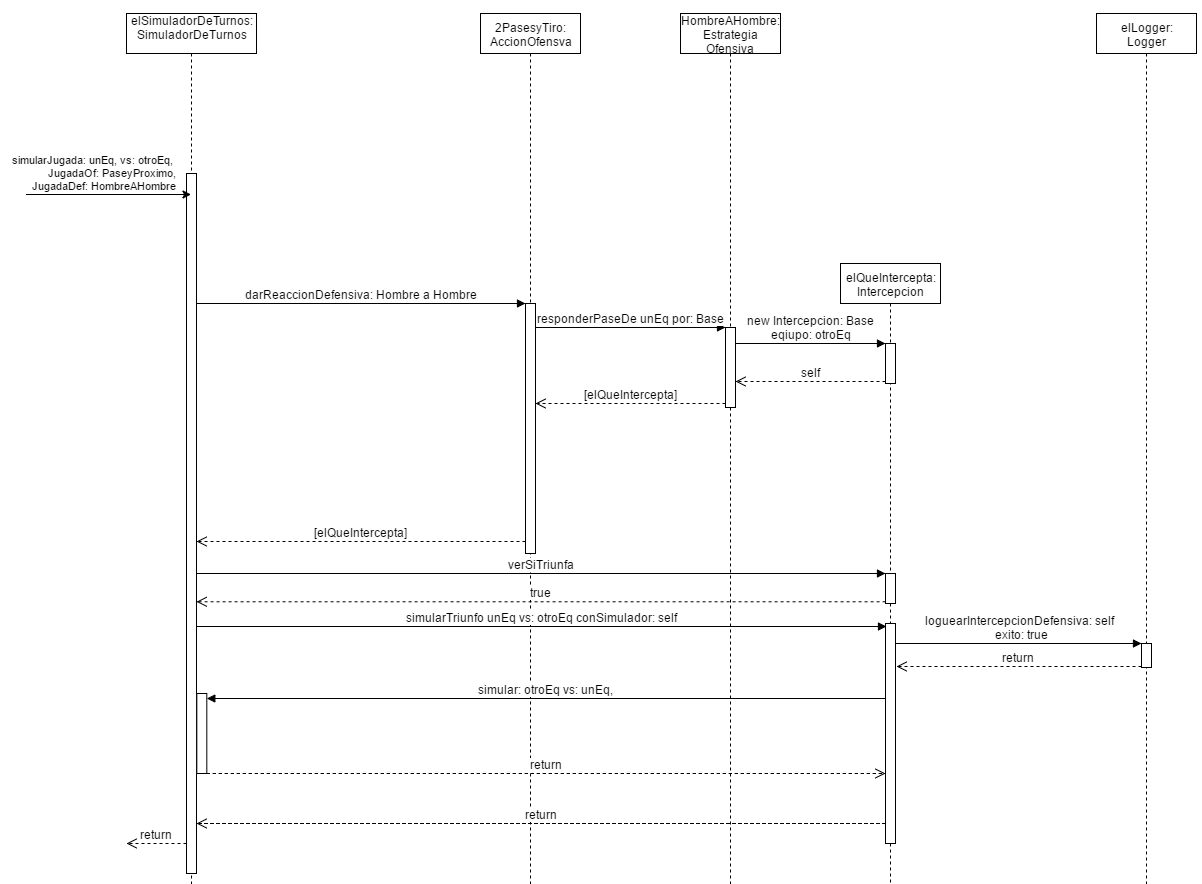
\includegraphics[width=\textwidth]{imgs/PaseFallido.png}

\subsection{Tiro Exitoso}

El siguiente diagrama muestra una secuencia de mensajes de un tiro que es exitoso. Esta secuencia estará en las simulaciones del simuladorDeTurno.

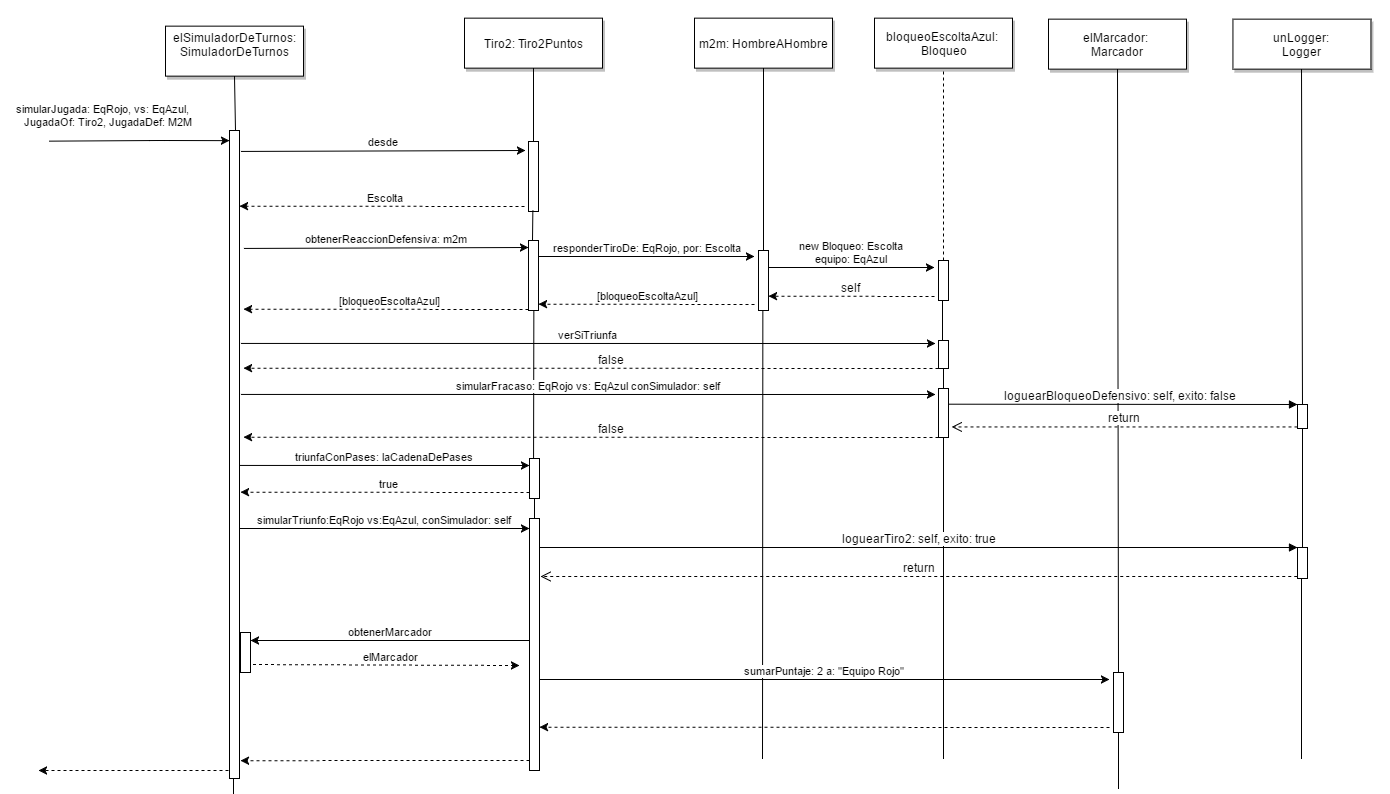
\includegraphics[width=\textwidth]{imgs/TiroExitoso.png}

\subsection{Tiro Fallido}

Análogamente para el Tiro Fallido

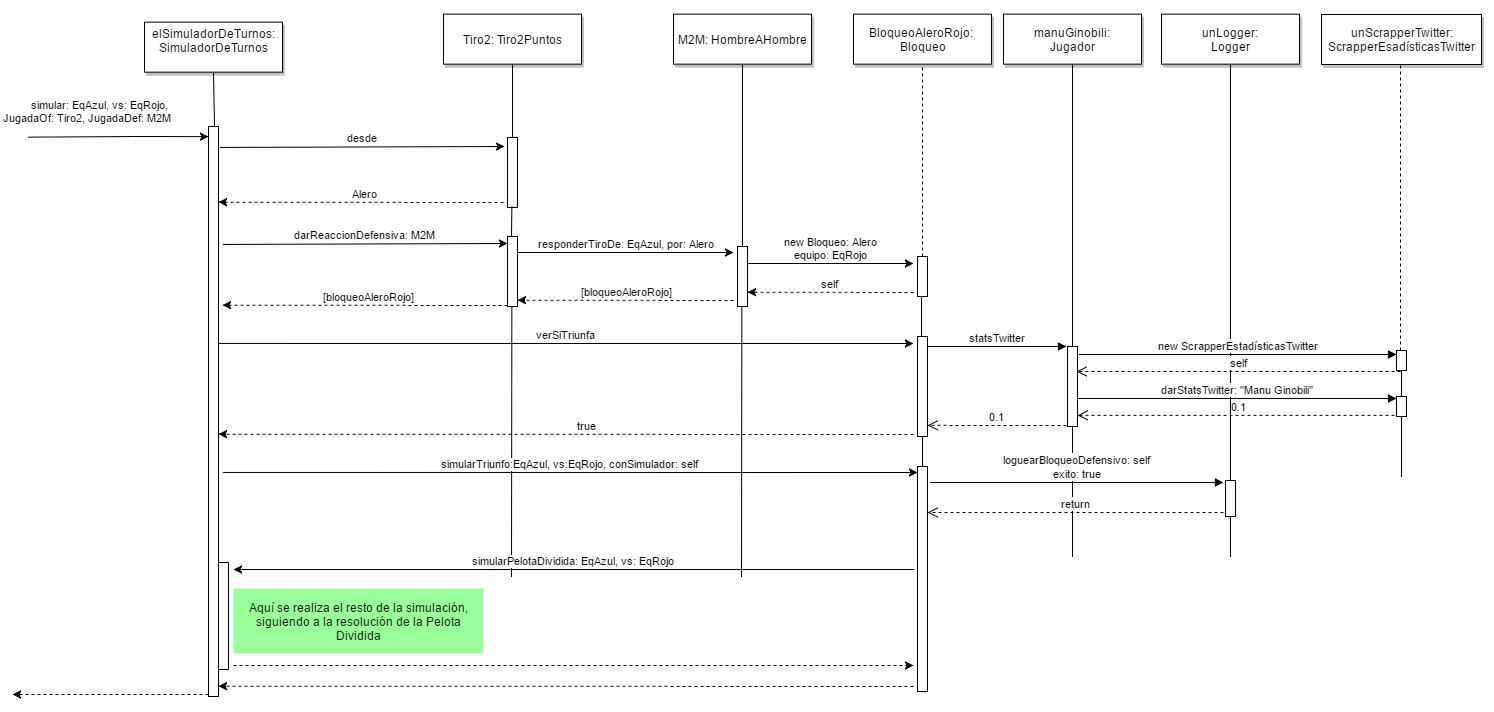
\includegraphics[width=\textwidth]{imgs/TiroFallido.png}

\subsection{Pelota Dividida}
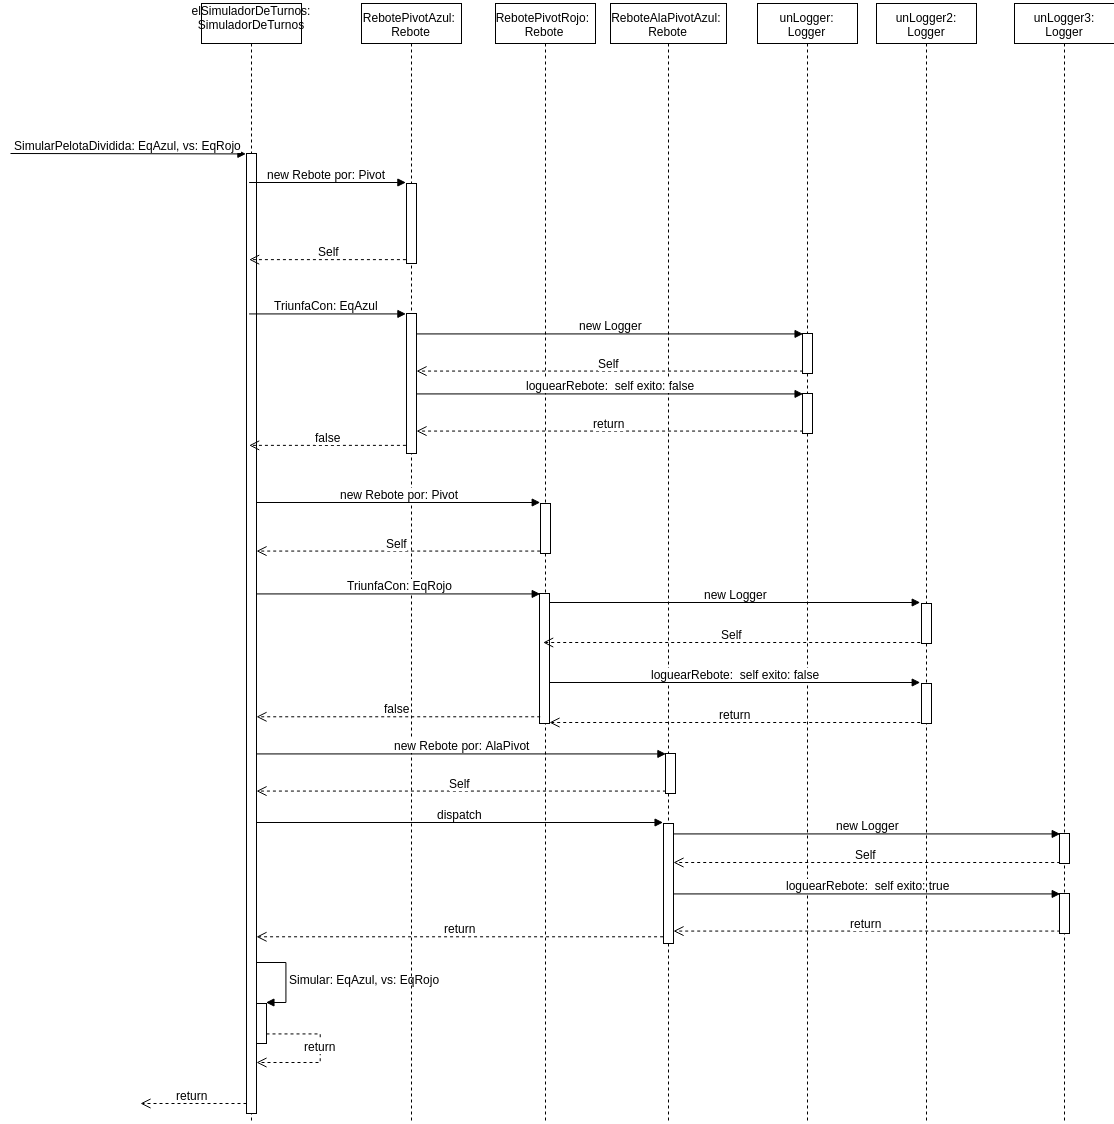
\includegraphics[width=\textwidth]{imgs/PelotaDivididaSecuencia.png}

\subsection{Colectiva Externa de 3}

El siguiente diagrama muestra un escenario donde en una jugada el equipo atacante (unEq) hace dos pases y un tiro y encesta, teneiendo como estrategia Colectiva Externa de k pases.

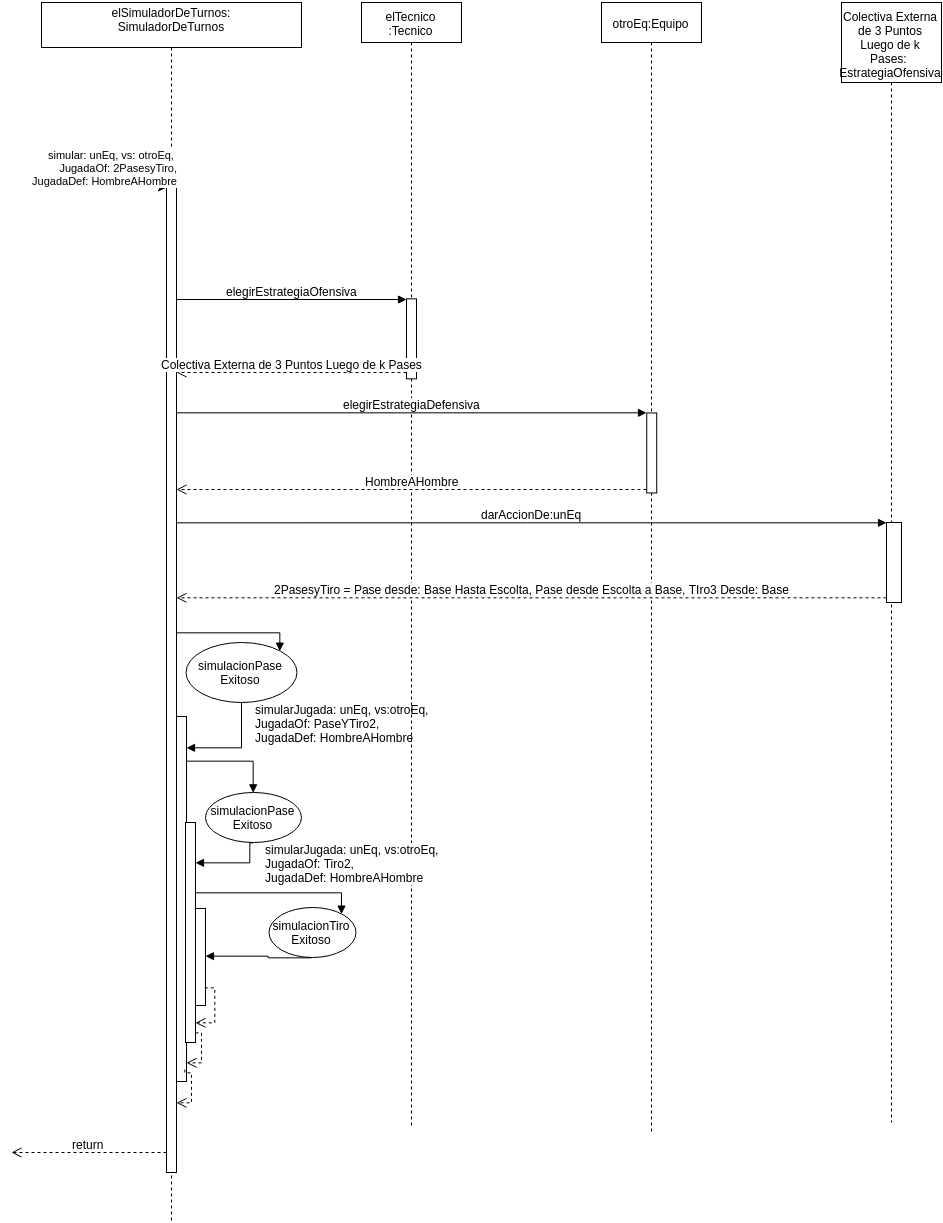
\includegraphics[width=\textwidth]{imgs/colectivaExternaDe3Secuencia.png}

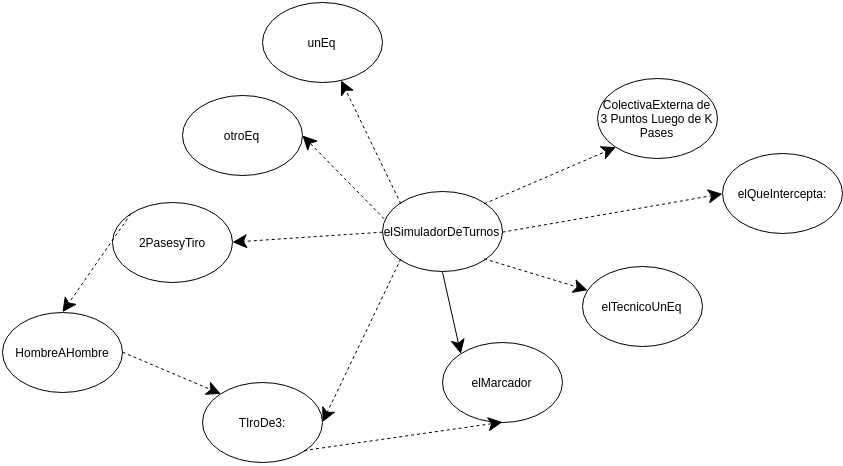
\includegraphics[width=\textwidth]{imgs/colectivaExternaDe3Objetos.png}

\subsection{Contraataque}
El siguiente diagrama muestra un escenario donde en una jugada el equipo atacante (eqAzul) hace un pase do forma exitosa, en el segundo pase es interceptado por el otro equipo y este ultimo tira al aro encestando sumando 2 puntos al marcador para su equipo.
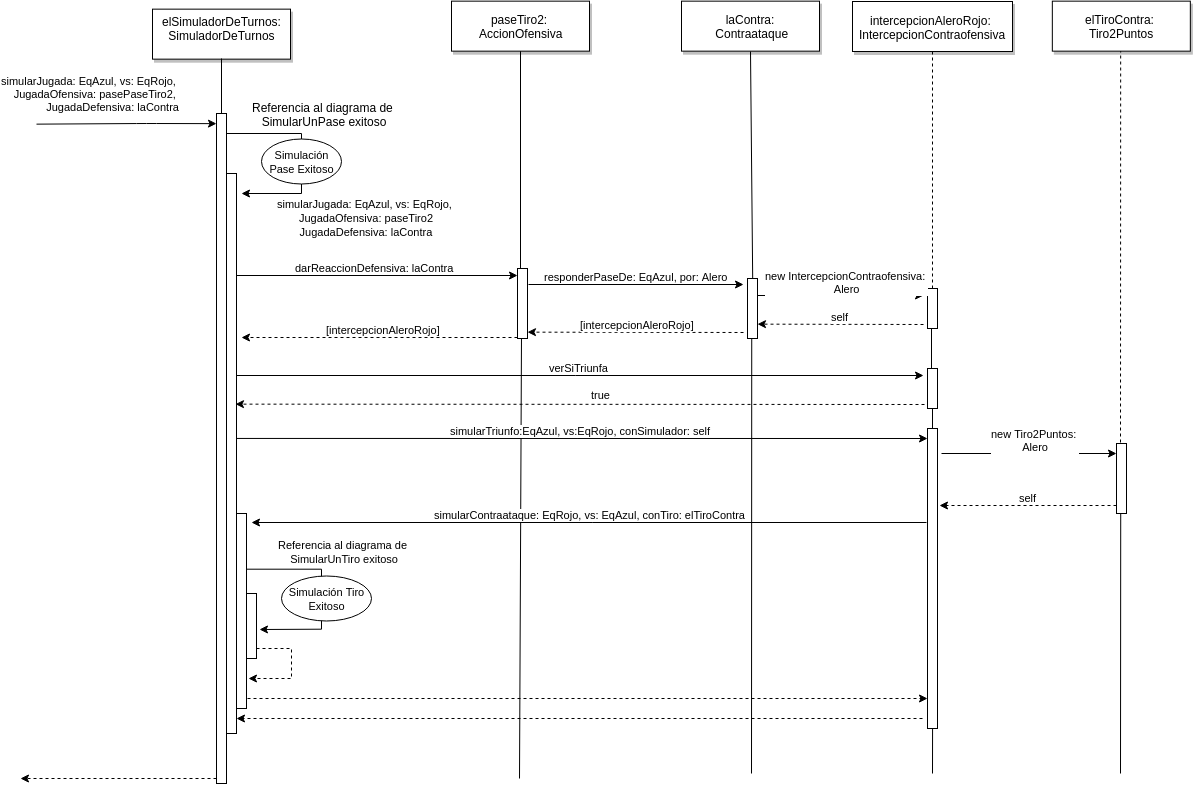
\includegraphics[width=\textwidth]{imgs/ContraataqueSecuencia.png}


